\section{Related Work}

\subsection{Commonsense Generation Tasks}
% Compared with \textit{discriminative} task, commonsense \textit{generative} task is more 
% challenging in composing sentences from scratch, which is considered as a significant 
% milestone of human development~\citep{tincoff1999, moore}. 

We mainly focus on $\mathcal{ART}$ and \textit{RocStory} datasets in this paper because they
naturally include both of commonsense \textit{generative} task and \textit{discriminative} task.
To solve the $\alpha$\textit{NLG} task, ~\citet{Bhagavatula2020Abductive} incorporate GPT-2~\citep{gpt2} 
with events commonsense knowledge generated by $\mathbb{COMET}$~\citep{comet}. 
~\citet{grf} firstly extract a knowledge subgraph from ConceptNet according to the given context,
then they perform graph encoding and reasoning on the extracted subgraph to obtain the necessary
knowledge information. ~\citet{DBLP:journals/tacl/GuanHHZZ20} instead implicitly introduced knowledge 
to the pre-trained language model by post-training on the knowledge-augmented data, which is constructed
by filling the template using triples from ConceptNet and ATOMIC. 
Our work is orthogonal to their work in two ways. i) Instead of resorting
to external commonsense knowledge source, we exploit the implicit commonsense knowledge~\citep{DBLP:conf/nips/TalmorTCGB20,DBLP:conf/emnlp/PetroniRRLBWM19,DBLP:conf/emnlp/DavisonFR19}
in large pre-trained language model. ii) We optimize the generative model by explicitly taking
the underlying goal as object, which is omiited in the mentioned previous work.
\begin{figure*}[ht]
    \centering
    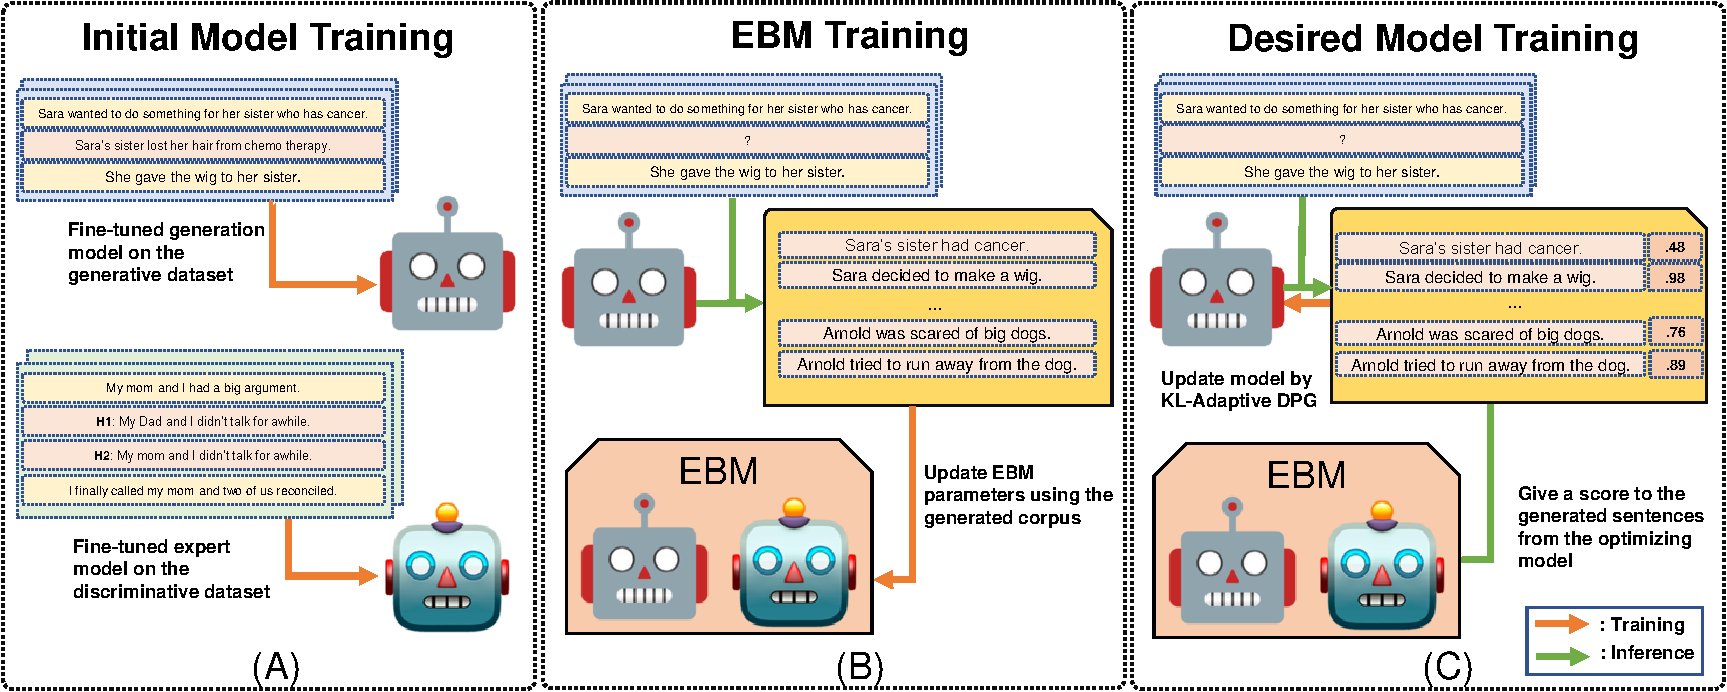
\includegraphics[width=1.0\textwidth]{figs/overview_graph.pdf}
    \caption{The training stages overview of $\mathcal{COSER}$, taking $\mathcal{ART}$ as example. 
    \textbf{(A)}: We firstly train the generative model and the expert model on their corresponding datasets.
    \textbf{(B)}: We sample sentences from the generation model as a corpus to train an EBM.
    \textbf{(C)}: The trained EBM scores each sentences generated by the generation model and instructs it
    for better generation. We implement this idea by formalizing the task in reinforcement learning setting
    and using the KL-Adaptive DPG algorithm.
    }
    \label{fig:overview}
\end{figure*}

\subsection{Controlled Text Generation}

Common automatic evaluation metrics for natural text generation(e.g., BLEU, ROUGE, etc) cannot 
directly nor fully access the underlying goal of specific tasks~\citep{DBLP:journals/corr/BengioVJS15}.
Therefore, people try to steer an autoregressive sequential model towards optimizing global reward over 
the generated text according to the task, including actor critic algorithm for Abstrative Summarization~\citep{DBLP:journals/corr/BahdanauBXGLPCB16},
Image Captioning~\citep{DBLP:journals/corr/LiuZYG016} and Machine Translation~\citep{DBLP:journals/corr/RanzatoCAZ15}.
To the best of our knowledge, we are the first one to alleviate this discrepency issue in commonsense
generation tasks. One might find that our work is similar to a GAN setting~\citep{DBLP:journals/corr/YuZWY16,DBLP:conf/icml/ZhangGFCHSC17}.
Besides consisting of a generative and a discriminative(expert) model, $\mathcal{COSER}$ is different from GAN
in the sense that the expert model is freezed during post-training.

\subsection{Energy-Based Model for Text Generation}

Energy-Based Models(EBM)~\citep{hintonebm,LeCun06atutorial,DBLP:journals/corr/RanzatoCAZ15,DBLP:conf/iclr/DengBOSR20}
are learning frameworks with decades of history. EBM provides a flexible and rich mechanism for specifying
models. EBM attracted a lot of attention in recent work, including
~\citet{DBLP:journals/corr/abs-1909-07063} and ~\citet{DBLP:conf/iclr/DengBOSR20}, who augment a standard
autoregressive LM with an additional global factor. ~\citet{dpg} treat a desired optimal language model under
specific constraints(e.g., token or sentiment) as EBM and then train an autoregressive LM through an adaptive
distributional variant of Policy Gradient. Inspired by their work, we augment the generative model with the
evaluation score from the expert model in order to generate more coherent and make-sense text within the context.
